\section{Learning Compact Boolean Networks} \label{sec:method}

In this section, we introduce our  methods to learn compact and accurate Boolean networks. 
We first present an efficient connection learning strategy in \cref{sec:learning_connectivity}, which is based on a novel parameterization of Boolean neurons
 that aggregates information from multiple connections, and an adaptive resampling strategy to continuously explore new connections.
Next, we present a compact convolutional Boolean architecture in \cref{sec:conv_without_trees}, replacing tree structures with single-operation
 kernels enabled by connection learning.
Finally, we introduce an adaptive discretization strategy in \cref{sec:adaptive_discretization}, progressively discretizing network layers during training to
reduce the accuracy drop.
\begin{figure*}[t]
\noindent\hbox to \textwidth{%
  \hfil
  \begin{subfigure}[t]{0.23\textwidth}
    \centering
    \resizebox{.7\linewidth}{!}{%
      \input{figures/single_input_gate.tikz}
    }
    \caption{Fixed connection. Each neuron observes two inputs.}
    \label{fig:conn-a}
  \end{subfigure}
  \hfil
  \begin{subfigure}[t]{0.23\textwidth}
    \centering
    \resizebox{.7\linewidth}{!}{%
      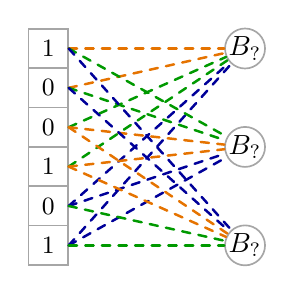
\begin{tikzpicture}[
  x=1cm,y=1cm,
  neuron/.style={circle,draw=gray!70,fill=white,minimum size=5mm,inner sep=0pt,line width=0.6pt},
  bitbox/.style={draw=gray!70,fill=white,minimum size=5mm,inner sep=0pt,line width=0.6pt,font=\small},
  worange/.style={orange!90!black, line width=0.9pt, dashed, line cap=round},
  wblue/.style={blue!60!black, line width=0.9pt, dashed, line cap=round},
  wgreen/.style={green!60!black, line width=0.9pt, dashed, line cap=round},
  lab/.style={font=\scriptsize}
]

\def\xin{0}
\def\xhA{2.5}
\def\xout{5.0}

\foreach \i/\y/\b in {1/2.5/1,2/2.0/0,3/1.5/0,4/1.0/1,5/0.5/0,6/0.0/1}{
  \node[bitbox] (in\i) at (\xin,\y) {\b};
}

\foreach \i/\y in {1/2.5,2/1.25,3/0.0}{
  \node[neuron] (hA\i) at (\xhA,\y) {$B_?$};
}

\draw[worange] (in1.east) -- (hA1);
\draw[worange] (in2.east) -- (hA1);
\draw[wgreen] (in3.east) -- (hA1);
\draw[wgreen] (in4.east) -- (hA1);
\draw[wblue] (in5.east) -- (hA1);
\draw[wblue] (in6.east) -- (hA1);
\draw[wgreen] (in1.east) -- (hA2);
\draw[wgreen] (in2.east) -- (hA2);
\draw[worange] (in3.east) -- (hA2);
\draw[worange] (in4.east) -- (hA2);
\draw[wblue] (in5.east) -- (hA2);
\draw[wblue] (in6.east) -- (hA2);
\draw[wblue] (in1.east) -- (hA3);
\draw[wblue] (in2.east) -- (hA3);
\draw[worange] (in3.east) -- (hA3);
\draw[worange] (in4.east) -- (hA3);
\draw[wgreen] (in5.east) -- (hA3);
\draw[wgreen] (in6.east) -- (hA3);


\end{tikzpicture}

    }
    \caption{Proposed parameterization. Every neuron aggregates multiple input pairs.}
    \label{fig:conn-b}
  \end{subfigure}
  \hfil
  \begin{subfigure}[t]{0.23\textwidth}
    \centering
    \resizebox{.7\linewidth}{!}{%
      
\begin{tikzpicture}[
  font=\large,
  gate/.style={draw=#1, line width=1.2pt, fill=none, scale=1.25},
  plus/.style={font=\Large},
  w/.style={font=\large},
]
\colorlet{myorange}{orange!90!black}
\colorlet{mygreen}{green!60!black}
\colorlet{myblue}{blue!60!black}

\def\dx{-0.8}
\def\yA{3}
\def\yB{0}

\coordinate (r1a) at (0,\yA);
\coordinate (r1b) at (2.5,\yA);
\coordinate (r1c) at (5,\yA);

\node[nand gate US, logic gate inputs=nn, gate=myorange] (A1) at (r1a) {$B_3$};
\node[xor  gate US, logic gate inputs=nn, gate=myorange] (B1) at (r1b) {$B_7$};
\node[or   gate US, logic gate inputs=nn, gate=myorange] (C1) at (r1c) {$B_9$};

\node[plus] at ($(A1)!0.5!(B1) + (0,0.05)$) {$+$};
\node[plus] at ($(B1)!0.5!(C1) + (0,0.05)$) {$+$};

\node[w, text=myorange] at ($(A1)+(0,\dx)$) {0.7};
\node[w, text=myorange] at ($(B1)+(0,\dx)$) {0.2};
\node[w, text=myorange] at ($(C1)+(0,\dx)$) {0.1};

\coordinate (r2a) at (0,\yB);
\coordinate (r2b) at (2.5,\yB);
\coordinate (r2c) at (5,\yB);

\node[nand gate US, logic gate inputs=nn, gate=myorange] (A2) at (r2a) {$B_3$};
\node[xor  gate US, logic gate inputs=nn, gate=myblue]   (B2) at (r2b) {$B_7$};
\node[or   gate US, logic gate inputs=nn, gate=mygreen]  (C2) at (r2c) {$B_9$};

\node[plus] at ($(A2)!0.5!(B2) + (0,0.05)$) {$+$};
\node[plus] at ($(B2)!0.5!(C2) + (0,0.05)$) {$+$};

\node[w, text=myorange] at ($(A2)+(0,\dx)$) {0.7};
\node[w, text=myblue]   at ($(B2)+(0,\dx)$) {0.2};
\node[w, text=mygreen]  at ($(C2)+(0,\dx)$) {0.1};

\end{tikzpicture}


    }
    \caption{Aggregation in fixed connection (up) and the proposed method (down).}
    \label{fig:conn-c}
  \end{subfigure}
  \hfil
  \begin{subfigure}[t]{0.23\textwidth}
    \centering
    \resizebox{.7\linewidth}{!}{%
      \begin{tikzpicture}[
  x=1cm,y=1cm,
  wire/.style={draw=gray!65,line width=0.6pt},
  bitbox/.style={draw=gray!70,fill=white,minimum size=5mm,inner sep=0pt,line width=0.6pt,font=\small},
  lbl/.style={font=\scriptsize}
]

\def\xin{0}
\foreach \i/\y/\b in {1/2.5/1,2/2.0/0,3/1.5/0,4/1.0/1,5/0.5/0,6/0.0/1}{
  \node[bitbox] (in\i) at (\xin,\y) {\b};
}

\def\xgate{2.5}
\node[nand gate US, draw=gray!70, logic gate inputs=nn, scale=0.85] (g1) at (\xgate,2.5) {$B_3$};
\node[xor gate US, draw=gray!70, logic gate inputs=nn, scale=0.85] (g2) at (\xgate,1.25) {$B_7$};
\node[or gate US, draw=gray!70, logic gate inputs=nn, scale=0.85] (g3) at (\xgate,0.0) {$B_9$};

\draw[wire] (in5.east) -- (g1.input 1);
\draw[wire] (in6.east) -- (g1.input 2);

\draw[wire] (in1.east) -- (g2.input 1);
\draw[wire] (in2.east) -- (g2.input 2);

\draw[wire] (in3.east) -- (g3.input 1);
\draw[wire] (in4.east) -- (g3.input 2);

\end{tikzpicture}

    }
    \caption{After discretization, only one input pair and Boolean operation remain.}
    \label{fig:conn-d}
  \end{subfigure}
  \hfil
}
\caption{Comparison between the parameterization with fixed connections (literature) and the proposed parameterization.}
\label{fig:conn-all}
\end{figure*}


\subsection{Efficient Connection Learning} \label{sec:learning_connectivity}
We modify the parameterization in \cref{eq:relaxation} 
to allow connection learning as follows. Instead of 
parameterizing neurons as a weighted aggregation 
of sixteen Boolean operations with the same inputs, 
we assign different inputs to different Boolean operations.
Specifically, 
let $\vx \in [0,1]^d$ be the vector representing the $d$ neurons in the $\ell$-th layer. 
For a neuron in the $(\ell+1)$-th layer, we parameterize it as  
\begin{equation} %
  \tilde{f^c}(\vx; \vk, \vp, \vq) = \sum_{i=1}^{16} \frac{\exp(\vw_i)}{\sum_{j=1}^{16} \exp(\vw_j)} B_{\vk_i}^c(\vx_{\vp_i}, \vx_{\vq_i}),
\end{equation}
where $\vk \in \{1, \dots, 16\}^{16}$ are indices denoting the Boolean operations, and $\vp, \vq \in \{1,\dots, d\}^{16}$
are indices denoting the two input neurons from the $\ell$-th layer, respectively.
At the beginning of training, $(\vk, \vp, \vq)$ can be sampled uniformly at random or follow any specific assignments. See \cref{fig:conn-all} for an illustration of the  parameterization. 


For each neuron, the optimal combination of inputs and Boolean function might not be included
in the initial assignment. To learn better combinations, we propose an adaptive 
resampling strategy.
The high-level idea is: once a neuron becomes ``stable'' during training, 
we resample its $(\vk, \vp, \vq)$ candidates to explore new combinations.
We measure the stability of a neuron by monitoring 
its  weight entropy, defined as:
\begin{equation*}
  h(\vw) = - \sum_{i=1}^{16} \tilde{\vw}_i \log \tilde{\vw}_i, \text{ where } \tilde{\vw}_i = \frac{\exp(\vw_i)}{\sum_{j=1}^{16} \exp(\vw_j)}.
\end{equation*}
The weight entropy equals zero if and only if one element in the normalized weight $\tilde{\vw}$ equals one, indicating that the neuron is represented by a single $(\vk_i, \vp_i, \vq_i)$ triple, and reaches its maximum when all elements in $\tilde{\vw}$ are equal, indicating that the neuron is an equal mixture of all $(\vk_i, \vp_i, \vq_i)$ triples.
We track the exponential moving average (EMA) of the weight entropy 
for each neuron individually.
 When the EMA of $h(\vw)$ for a neuron 
 converges, its weight vector $\vw$ can have three possible states:
(i) dominated by a single triple $(\vk_i, \vp_i, \vq_i)$ , i.e., $\exists i^*, \tilde{\vw}_{i^*} \ge 0.95$;
(ii) dispersed, i.e., $\max_i \vw_i \le 0.4$;
(iii) concentrated without a dominant triple. 
For (i), further training of the neuron is unlikely to improve the discretized network unless the dominant triple is replaced, so we resample all $(\vk_i, \vp_i, \vq_i)$ except the dominant one to explore new combinations.
For (ii), the neuron fails to find a useful triple, thus we resample all $(\vk_i, \vp_i, \vq_i)$ to restart its learning. Neurons falling into the third case are not changed since they are still learning. 
We refer to the  pseudocode in \cref{alg:resampling} for further details.
We note that after training, most neurons (frequently over 90\%)
 empirically end up in the first case, indicating that they have learned meaningful patterns expressed by a single dominant connection and Boolean function.

\begin{algorithm}[tb]
  \caption{Adaptive Resampling}
  \label{alg:resampling}
  \begin{algorithmic}
    \STATE {\bfseries Input:} initial neuron weight $\vw \in \sR^{16}$, weight update function $\STEP$, EMA momentum $\rho$, stability threshold $\epsilon$, patience $T$, \#triples per neuron $K=16$.
    \STATE {\bfseries Output:} trained neuron weight $\vw$

    \STATE $\mu \gets 0$, $c \gets 0$
    \REPEAT
      \STATE $\vw \leftarrow \STEP(\vw)$
      \STATE $h \gets - \sum_{i=1}^{K} \tilde{\vw}_i \log \tilde{\vw}_i, \text{ where } \tilde{\vw}_i = \frac{\exp(\vw_i)}{\sum_j \exp(\vw_j)}$
      \STATE Increase $c$ by 1 if $|\mu - h| \le \epsilon$, else set $c \gets 0$
      \STATE $\mu \gets \rho \mu + (1-\rho) h$
      \IF{$c \ge T$}
        \STATE dominated $\gets$ check if $\exists i^*, \tilde{\vw}_{i^*} \ge 0.95$
        \STATE dispersed $\gets$ check if $\max_i \tilde{\vw}_i \le 0.4$
        \IF{dominated}
          \STATE resample all $(\vk_i, \vp_i, \vq_i)$ except the dominant one
          \STATE reset $\vw$ such that $\tilde{\vw}_{i^*}=0.9$ and $\tilde{\vw}_j=\frac{0.1}{K-1}$ for $j \neq i^*$
        \ELSIF{dispersed}
          \STATE resample all $(\vk_i, \vp_i, \vq_i)$
          \STATE reset $\vw$ such that $\tilde{\vw}_i=\frac{1}{K}$ for all $i$
        \ENDIF
      \ENDIF
      \STATE reset $c \gets 0$ if resampling is performed
    \UNTIL{training ends}
  \end{algorithmic}
\end{algorithm}

We remark on the relation to prior works and the overhead of the proposed method.
As mentioned in \cref{sec:intro}, 
\citet{petersen2022deep,petersen2024convolutional} and \citet{ruttgers2025light}
randomly sample the connection and keep it fixed during training. 
 To allow learning connections,  \citet{bacellar2024differentiable} and \citet{fojcik2025lilogic} 
propose to parameterize the connections with additional weight matrices.
A Boolean layer with $\din$ input neurons and $\dout$ 
output neurons additionally maintains a weight matrix $W_{\text{link}} \in \sR^{\din \times \dout}$.
However, such large matrices are 
 often impractical: for a typical medium-sized model in  \citet{petersen2024convolutional}, $W_{\text{link}}$ for a single 
 layer can consume over 3400 GB of memory. In contrast, our method learns the network connection without 
 additional 
 parameters.
 Nevertheless, compared to \citet{petersen2022deep,petersen2024convolutional}, it does introduce mild computational and memory overhead during training (but not at inference): EMAs are tracked (a scalar per neuron), 
 and resampling is performed periodically. However, these overheads are typically negligible compared to the overall training cost. 

\subsection{Convolution without Boolean Trees} \label{sec:conv_without_trees}
Convolution is a key component in floating-point neural networks 
to capture spatial features, especially for vision tasks.
A natural and easy way to construct convolutional layers in Boolean networks 
is to take a single Boolean operation
 as the convolutional kernel. 
However, such kernels under fixed connections only observe two inputs from 
the receptive field.   
With the design in  \cref{sec:learning_connectivity},  this does not constitute a problem:
 a convolutional kernel 
  learns to extract important information from the full receptive field by aggregating 
  multiple input pairs during training, thus the kernel can observe up to 32 distinct inputs from the receptive field. As a result, we can learn a compact convolutional Boolean network based on single-operation kernels.


  In contrast, the convolutional kernels in \citet{petersen2024convolutional}
are built on Boolean trees.  Specifically, $2^{d-1}$ neurons sampled 
from the receptive field are fed into a binary Boolean tree of depth $d$, and then every node in the tree 
is learned with the relaxation in \cref{eq:relaxation}. Such tree structure has two main issues. First,
 the number of Boolean operations per layer grows exponentially with the tree depth $d$, leading to high inference costs.
  Second, the hierarchical structure of binary trees introduces sequential dependencies that limit parallelism during both 
  forward and backward passes. As we later demonstrate empirically in \cref{sec:experiments},
  our method can learn much smaller convolutional Boolean networks with higher accuracies.

\subsection{Adaptive Discretization} \label{sec:adaptive_discretization}

\begin{figure}
    \centering
    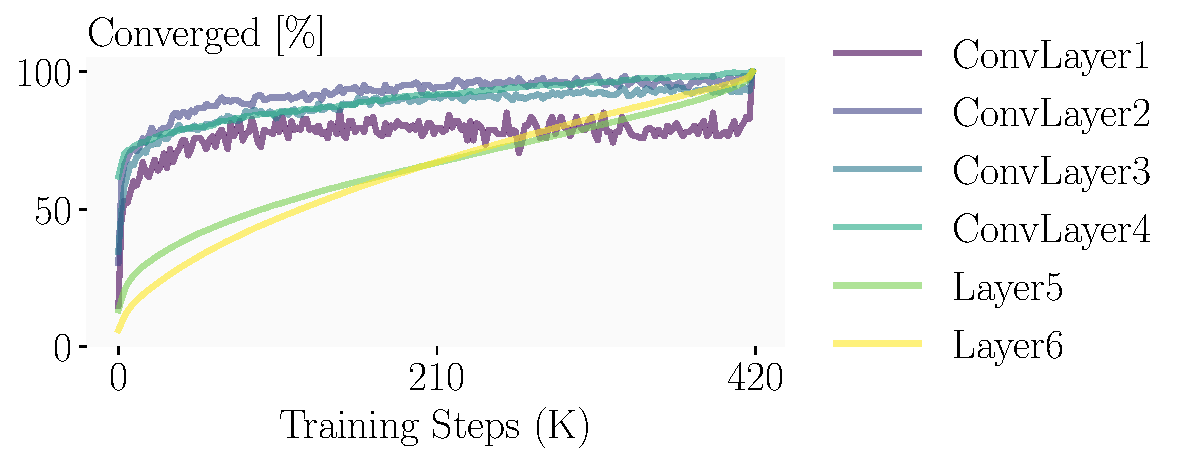
\includegraphics[width=0.95\columnwidth]{figures/row_argmax_difference}
    \caption{Convergence speed of different layers.}
    \label{fig:row_argmax_difference}
    \vspace{-1em}
\end{figure}

As introduced in \cref{sec:background}, after training, the network 
is discretized to Boolean by replacing all relaxed neurons with their dominant Boolean operation at once.  
However, such  training paradigm ignores the discrepancy 
between the continuous and Boolean networks, and thus leads to a systematic accuracy drop after discretization.
We shall address the discretization issue in this subsection. 

During training, convolutional layers of the network tend to converge faster than the non-convolutional layers. We measure the ratio of neurons that have the same dominant $(\vk_i, \vp_i, \vq_i)$ triple as the final discretized network. As shown in \cref{fig:row_argmax_difference}, convolutional layers converge much faster than non-convolutional layers. Further, convolutional layers tend to be less stable, \eg the first convolutional layer stops improving when roughly 80\% neurons converge, while non-convolutional layers converge more steadily.
Based on these observations, 
we propose to adaptively discretize (and thus freeze) the network progressively from shallow to deep layers during training.
 Specifically, we monitor the convergence of each layer using the average weight entropy and EMAs, similar to \cref{sec:learning_connectivity}.
Once the first layer converges, we immediately discretize it by \cref{eq:discretization}  (thus stop training it) and continue training the
subsequent layers. We proceed layer-wise in this manner for all convolutional layers, and then continue training the
non-convolutional layers in their relaxed form until the end. A pseudocode is provided as \cref{alg:discretization}.
The progressive discretization  forces the layers to adapt to Boolean inputs during training. As a result,   the network suffers less from the accuracy drop caused by discretization.



We remark that
 \citet{kim2023deep} and \citet{yousefi2025mind} attempt to
 mitigate the discretization issue as well, but via injecting noise during training.
However, the injected noise distribution does not accurately reflect the true distribution of the discretization error, and thus fails to guide the training towards better solutions (c.f. \cref{sec:exp_discretization}).



\begin{algorithm}[tb]
  \caption{Adaptive Discretization}
  \label{alg:discretization}
  \begin{algorithmic}
    \STATE {\bfseries Input:} weights $\mW$ returned by \cref{alg:resampling}, weight update function $\STEP$, EMA momentum $\rho$, stability threshold $\epsilon$, patience $T$.
    \STATE {\bfseries Output:} discretized Boolean network
    \REPEAT
      \STATE $\mW \gets \STEP(\mW)$
      \STATE $l \gets$ the first non-discretized layer
      \STATE Initialize $\mu_l \gets 0$, $c_l \gets 0$ if not initialized
      \STATE Compute average weight entropy $h_l$
      \STATE Increase $c_l$ by 1 if $|\mu_l - h_l| \le \epsilon$, else set $c_l \gets 0$
      \STATE $\mu_l \gets \rho \mu_l + (1-\rho) h_l$
      \IF{$c_l \ge T$}
        \STATE Freeze and discretize layer $l$ using \cref{eq:discretization}
        \STATE Mark layer $l$ as discretized
      \ENDIF
    \UNTIL{training ends}
  \end{algorithmic}
\end{algorithm}
